\documentclass[useAMS,usenatbib,onecolumn]{mnras}

\usepackage{graphicx}
\usepackage{listings}
\lstset{
  basicstyle=\ttfamily,
  mathescape
}

\begin{document}

\noindent\makebox[\textwidth][c]{\Large\bfseries Nested Sampling}

\section{Intro and Motivation}

Working in a Bayesian framework, we start with,
\begin{equation}
    P(\theta | D, M) = \frac{\mathcal{L(D | \theta, M)} \pi(\theta)}{\mathcal{Z}}
\end{equation}

Where we define a likelihood function along with the prior on our parameters. From these, we want to compute either the posterior, $P(\theta | D, M)$, or the evidence,

\begin{equation}
    \mathcal{Z} = \int \mathcal{L}(\theta) \pi(\theta) d\theta
\end{equation}

Most traditional methods (e.g. MCMC) focus on finding the posterior. In MCMC we generate samples {\bf proportional} to the posterior. Once we have enough samples, we claim that

\begin{equation}
    P(\theta | D, M) \sim \hat{P}(\theta) = \frac{\sum_{i=1}^{N} \delta(\theta_i)}{N}
\end{equation}

\noindent where $\delta(\theta_i)$ is the delta function at the position of the sample in parameter space, and we normalize to get a posterior that integrates to 1.


However the posterior is not the only output. We can rewrite Bayes Theorem as,
\begin{equation}
    P(\theta)d\theta \times \mathcal{Z} = \mathcal{L(\theta)} \times \pi(\theta) d\theta
\end{equation}

\noindent which makes it clear that, given the likelihood and prior there are two possible outputs.

\subsection{Why we can't get the evidence easily from the posterior?}

EEK?


\subsection{What we can do with the evidence}

Model selection (compare Bayes factors)

\section{Nested Sampling}

\subsection{Theory}

Nested sampling tries to estimate the evidence (model evidence, marginal likelihood).

\begin{equation}
    \mathcal{Z} = \int \mathcal{L}(\theta) \pi(\theta) d\theta
    \label{eq:evidence}
\end{equation}

This is hard, as the integral is over the multi dimensional domain of $\theta$. While simplistically, one might just evaluate this at a grid of positions, this becomes impractical once $\theta$ has more than a few dimensions. Nested Sampling does clever things to allow us to solve this integral.

First let's define,
\begin{equation}
    dX = \pi(\theta) d\theta
\end{equation}

\noindent this is the amount of prior mass in a small region of $\theta$ space ($\pi$ is a density, $d\theta$ is a volume). We can substitute this into our evidence equation (\autoref{eq:evidence}),

\begin{equation}
    \mathcal{Z} = \int \mathcal{L}(\theta) dX
\end{equation}


\noindent But we are still performing an multidimensional integral over $\theta$ space. Intuitively, I think of this as ranging over each dimension in that space in turn. However, there is no rule that governs the order in which we perform the summations. Let's sort our volume by the likelihood at each location, and define the prior mass as a function of likelihood,

\begin{equation}
    X(\lambda) = \int_{L(\theta) > \lambda} \pi(\theta) d\theta
\end{equation}

\noindent where $X$ is the total prior mass above a given likelihood, $\lambda$. Note that $X$ ranges from 1 (for $\lambda = 0$, as all locations have some positive likelihood) to $0$ (for $\lambda = \infty$, as there is no mass above this) . Note that $X$ is monotonically {\em decreasing} as $\lambda$ increases.
We can invert this mapping, and define $\mathcal{L}(X)$, the minimum likelihood in that mass range. Note that $\mathcal{L}$ is monotonically {\em decreasing} with $X$.
Large minimum likelihood, small volume. Small minimum likelihood, large volume.

With this mapping, we can recast the integral over $X$ space. We integrate over the total mass (0 to 1), taking the likelihood at that mass range,

\begin{equation}
    \mathcal{Z} = \int_0^1 \mathcal{L}(X) dX
    \label{eq:theory_final}
\end{equation}

Note that we could also phrase this as,

\begin{equation}
    \mathcal{Z} = \int_0^\infty X(\lambda) d\lambda
\end{equation}


\begin{figure}
     \begin{center}
     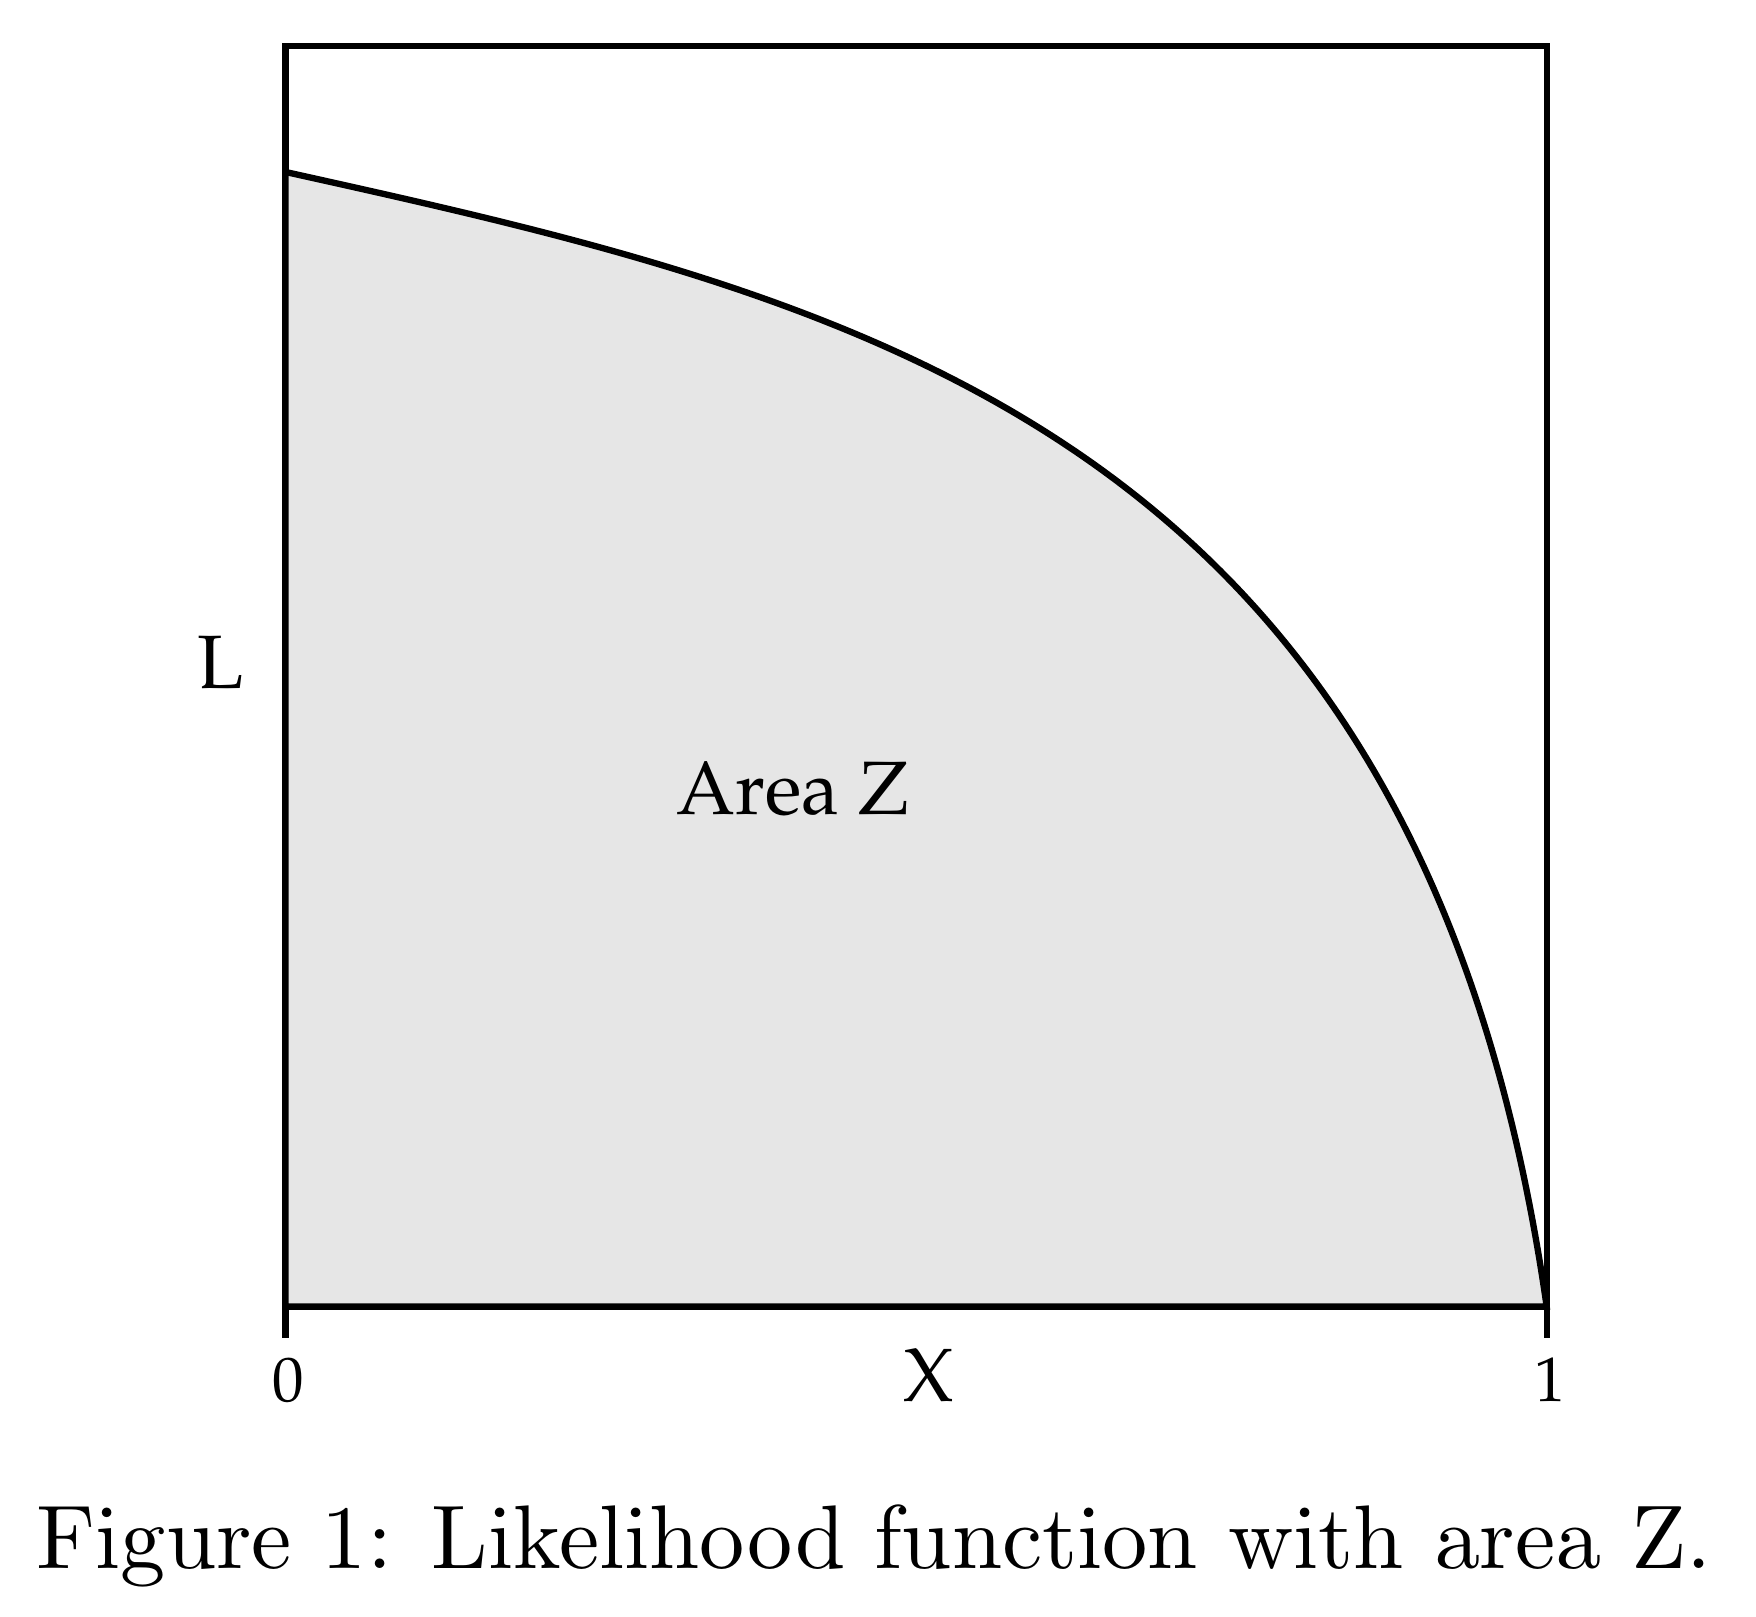
\includegraphics[width=0.5\textwidth]{plots/skilling2006_fig1.png}
     \caption{\
         Visual representation of \autoref{eq:theory_final}. We integrate the likelihood as a function of the amount of prior mass $X$ that has at least that likelihood, over all the prior mass.
     }
     \end{center}
\end{figure}

\subsection{Practical}

\begin{lstlisting}
N := the number of live-points
Randomly select N live-points $\theta_1$,...,$\theta_N$ from the prior. Assign their likelihoods, $\mathcal{L}_1,...,\mathcal{L}_N$.

Set $\mathcal{Z} = 0$, $X_0$ = 1
\end{lstlisting}

We start with all the space left to explore ($X_0 = 1$) and no evidence found ($\mathcal{Z} = 0$).

\begin{lstlisting}
For i in 1...:
    Find the live point with the lowest likelihood, $\mathcal{L}_i$.
    Set $X_i = \exp(-i / N)$
\end{lstlisting}

What can we say about any new point that we draw, given that $\mathcal{L}_i > \mathcal{L}_{i-1}$, or equivalently $X_i < X_{i-1}$? Well we know that $X_i = t_i X_{i-1}$ where $0 < t_i < 1$. In fact, $t_i \in {\rm Uniform}(0, 1)$. The mass is reduced by a constant fraction each step.

\begin{lstlisting}
    Set $w_i = X_{i-1} - X_i$
    $\mathcal{Z} += \mathcal{L}_i w_i$
\end{lstlisting}

Add the extra evidence, the likelihood multiplied by the width of the interval.

\begin{lstlisting}
    Then replace this lowest likelihood live point with one drawn from the prior, such that $\mathcal{L}(\theta) > \mathcal{L}_i$.
\end{lstlisting}





\section{Refs}

\cite{Speagle2020}
\cite{Skilling2006}

\url{https://ned.ipac.caltech.edu/level5/Sept13/Trotta/Trotta4.html}


\bibliographystyle{mnras}
\bibliography{/home/christopher/research/researchNotes/bibliography/astro}
\end{document}
